%=======================================================================
% Introdução
%=======================================================================
% Para a Introdução não ser o capítulo 1, usar:
%\chapter*{Introdução}
%\addcontentsline{toc}{chapter}{Introdução}
\chapter{Introdução}

%    - Descrição do problema (motivação) 
%    - Revisão do estado da arte 
%    * (qual a precisão dos sistemas existentes?)
%    - Breve descrição da proposta de trabalho

	Em meio a grande variedade de opções de produtos vindos do mundo inteiro para o consumidor brasileiro, a indústria nacional que é destinada à produção de bebidas passa por um momento de transformação de conceitos no qual a qualidade deve estar em destaque. Os rótulos têm uma grande influência na decisão de compra do consumidor final. Elementos como cores, formas, materiais, imagens  e a linguagem utilizada, podem trazer ao rótulo uma identidade única, influenciando em sentimentos, percepções e valores funcionais aos produtos, que auxiliam e atraem o consumidor na decisão de compra. Em sua maioria, contêm a identidade de uma marca, assim como informações relevantes ao produto, tal como funcionalidades, prazos de validade, avisos e etc. 
	 
	Quando um rótulo apresenta alguma deformidade na sua impressão ou fixação pode levar ao consumidor uma percepção de descuido ou sentimento pejorativo com relação ao produto, influenciando diretamente na sua decisão de compra. Com isso, as empresas do ramo procuram se desenvolver tecnologicamente com o intuito de minimizar essas deformidades. A solução geralmente adotada é a inspeção dos produtos, visando a eliminação daqueles fora de conformidade. Para isso, as pequenas empresas tendem a utilizar inspeção visual humana, que é lenta e não confiável, visto que não há uma tecnologia automatizada nacional e/ou com custo acessível para esse tipo de aplicação. Já para as empresas de grande porte, tende a ser viável a opção por tecnologias importadas, geralmente com alto valor de mercado. 
	 
    Uma das alterativas de inspeção automatizada disponíveis no mercado é a tecnologia da empresa alemã EVT (\textit{http://www.evt-web.com/}), que utiliza uma ferramenta CAD  (\textit{Computer-Aided Design}) para fazer a análise do rótulo através de imagens adquiridas em tempo-real. 
    As garrafas são submetidas a um processo de medição por imagens e caso não ocorra diferenças consideráveis entre a disposição do rótulo aplicado e um padrão pré-definido, a garrafa é aprovada por estar dentro dos padrões de qualidade da empresa. Um ponto negativo desse método é a necessidade de posicionar as garrafas com o rótulo virado para a câmera no momento da inspeção. Caso isso não ocorra, o sistema pode rejeitar garrafas com padrões de qualidade aceitáveis. Com vistas a evitar um posicionamento preciso das garrafas frente à câmera, alguns sistemas (\textit{https://www.ftsystem.com/english/}) utilizam mais de uma câmera, de forma a adquirir imagens de diversos ângulos da garrafa. Os sistemas comerciais  existentes possivelmente buscam, entre essas imagens, o melhor ângulo de observação de cada característica a ser inspecionada.
    
    O problema de inspeção de rótulos é pouco abordado na comunidade científica, não gerando resultados consistentes com o assunto quando, por exemplo, as palavras-chave \textit{bottle}, \textit{label} e \textit{inspection}, jargões técnicos usuais na área, são utilizadas nas ferramentas de procura do IEEEXplore e do Google Scholar. Até onde alcançou a pesquisa bibliográfica que embasa este trabalho, um único artigo foi encontrado com o propósito de inspeção de rótulos \cite{Lin:2013}.  
    
    Em \cite{Lin:2013} é proposto um sistema de inspeção baseado na utilização de quatro câmeras, que atuam simultaneamente, a fim de capturar imagens em torno do perímetro da garrafa. Essas quatro imagens são utilizadas para compor uma imagem panorâmica que, posteriormente, pode ser utilizada para comparação com uma panorâmica padrão (ainda que o artigo não avance até tal etapa). Para isso, os autores apresentam um modelo trigonométrico para compensação das distorções projetivas presentes em cada uma das cenas. Uma vez feitas essas compensações, as imagens são alinhadas por meio de um algoritmo de \textit{registro}, responsável por estimar o deslocamento relativo entre imagens. 
    
    A maneira de se compor uma imagem panorâmica (e, por hipótese, periódica) da superfície da garrafa possibilita que eventuais problemas de posicionamento dos rótulos possam ser detectados por alguma medida de similaridade; por exemplo, estatística, como a correlação. A formação de imagens panorâmicas é um tema amplamente abordado na literatura \cite{Lee:2001, Park:2013}. Entretanto, o modelo geométrico das aplicações usuais é geralmente o inverso do modelo geométrico da aplicação em questão. As aplicações tradicionais se configuram como uma câmera que é rotacionada em torno de um eixo de fixação, estando ela posicionada ao longo do raio de rotação e direcionada no sentido oposto ao eixo (ver Figura~\ref{fig:gp}~(a)). Na aplicação de inspeção de rótulos, a geometria do problema é similar, mas a câmera fica direcionada no sentido do eixo de rotação (ver Figura~\ref{fig:gp}~(b)).
    
\begin{figure}[ht]
    \centering
    \caption{Modelo geométrico de imagens panorâmicas.}    
    \begin{minipage}{\textwidth}
        \begin{tabular}{cc}
            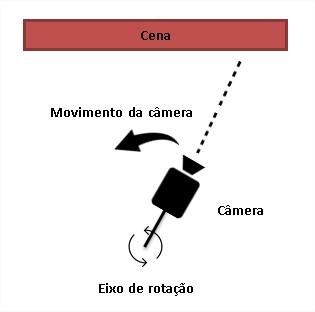
\includegraphics[width=.4\linewidth]{TCC/Imagens/panoramica_padrao.jpg} 
            &
            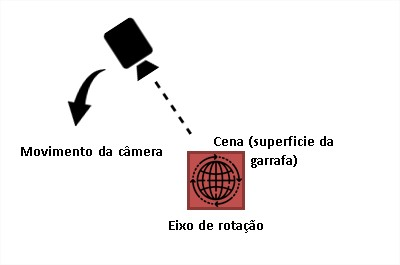
\includegraphics[width=.5\linewidth]{TCC/Imagens/panoramica_trabalho.jpg}
            \\
            (a) Aplicações típicas & (b) Aplicação de inspeção de rótulos.
        \end{tabular}
        \fonte{O autor (2020)}
    \end{minipage}
    \label{fig:gp}
\end{figure}
    
    Existem outras aplicações com essa mesma geometria, cujos autores propõem soluções semi-supervisionadas \cite{lee2000fast} ou propõem soluções de alto custo de hardware (baseadas em \textit{scanners} 3D) e de processamento \cite{Kovacs:2006}, enquanto as linhas de produção de bebidas produzem em velocidades típicas que variam de 2,5 a 15 garrafas por segundo. Além disso, as condições de aquisição em linhas de envase de bebidas são mais facilmente controladas e o produto sob inspeção possui uma geometria substancialmente mais simples que em \cite{lee2000fast,Kovacs:2006}, o que potencialmente possibilita o uso de técnicas igualmente mais simples (e portanto computacionalmente menos custosas) e com resultados mais confiáveis \cite{Park:2013}.
    
    O presente trabalho estuda a aplicação do método proposto em \cite{Lin:2013}, porém sem o uso de algoritmos de registro. Para tanto, o deslocamento entre as cenas é assumido conhecido, com base na posição das quatro câmeras. 
    
    O presente texto está dividido em cinco capítulos. Este primeiro Capítulo é introdutório e, na próxima seção, ainda são apresentados os objetivos do trabalho. O segundo Capítulo descreve a teoria necessária para realizar o mapeamento das distorções, compensações geométricas e a técnica utilizada por \cite{Lin:2013} para a montagem de um mosaico. O método proposto é apresentado no Capítulo 3. No Capítulo 4 são apresentados e discutidos os resultados obtidos. Por fim, o Capítulo 5 finaliza o trabalho.

	\section{Objetivos}
	
	\subsection*{Objetivo geral}
        Gerar uma imagem panorâmica da superfície de um objeto cilíndrico.
	\subsection*{Objetivos específicos} \label{sec:objetivos:especificos}
	\begin{enumerate}
		\item Investigar uma técnica potencialmente adequada à construção de imagens panorâmicas da superfície de garrafas;
		\item Avançar o conhecimento do Núcleo de Inovação e Desenvolvimento em Controle e Automação, da Universidade de Caxias do Sul, a respeito de técnicas de mosaico de imagens;
		\item Avançar o conhecimento do Núcleo de Inovação e Desenvolvimento em Controle e Automação, da Universidade de Caxias do Sul, na direção do desenvolvimento de um inspetor de rótulos para linhas de envase de bebidas.
	\end{enumerate}
